% -*- root: ../main.tex -*-
\chapter{Processo di Sviluppo}

\section{Domain Driven Design}
Il processo di sviluppo è stato guidato dalla filosofia data dal Domain Driven Design. La realizzazione di questo progetto costituisce, per i membri del team, un ottimo terreno di prova per mettere in campo molti degli aspetti di gestione propri di questo approccio.
    \subsection{Aspetti principali del DDD}
    Il Domain Driven Design è un approccio che si rivela ideale per la conduzione di progetti non banali che richiedono l'interazione di persone con background differenti. 
    L'obiettivo è quello di evitare gli errori comuni che tendono a verificarsi in mancanza di una buona gestione e comunicazione. Più che un pattern o un framework, il DDD è una filosofia che rappresenta una guida. 
    
    Il Domain Driven Design è un approccio operativo che tenta di uniformare il modello di dominio con l'artefatto generato, cercando di muovere concetti fondamentali per l'ambito all'interno del software e della documentazione, che dovranno quindi rispecchiare in dominio utilizzando il giusto linguaggio.
    Il classico approccio di standardizzazione delle pratiche di analisi e progettazione, tende a deviare il software lontano dal contesto di dominio. Questo rende il prodotto poco robusto e solo parzialmente coerente con l'ambito.
    Per questo il DDD non è vincolato ad una particolare tecnologia o pattern di design, favorendo lo sviluppo mirato caso per caso.
    Tenta di trasmettere i costanti cambiamenti del dominio nel prodotto mantenendo una dualità costante che consente di ottenere un prodotto più coerente e leggibile sia per il team che per il cliente. 
    
    Generalmente utilizzato per progetti sia di medie che di grandi dimensioni che evolvono nel tempo, non è una metodologia o un architettura. Può essere visto come un approccio che coinvolge più strati socio-tecnologici orizzontalmente, dal business ai vincoli implementativi fino alle buone pratiche di coding.
    
    
    
    Concetti chiave che DDD porta con sè:
    
        \begin{itemize}
        \item \textbf{Strategia}: ogni problema ha la sua soluzione, non esiste il famoso silver bullet, bisogna trovare il giusto approccio e non cercare di eccedere con eccessivi strumenti o tecniche ove non richiesti.
        Non tutte le parti del prodotto necessitano la stessa modellazione, applicare ogni feature dell' approccio DDD per tutti i problemi può portare a problemi peggiori.
        DDD impone di identificare e distinguere il \textbf{Core Domain}; la parte che detiene il business value maggiore e di dedicarvi più risorse e tempo.
        Mentre per le restanti parti, i \textbf{subdomain}, è possibile utilizzare un approccio più conservativo.
        
        \item \textbf{Learning}: forse il passo più critico per ottenere un prodotto di qualità. Il processo di apprendimento deve essere costante e continuativo, consentendo di diffondere un sapere condiviso che incentiva la comunicazione e agevola la costruzione di una soluzione coerente e coesa con la terminologia del dominio. 
        L'apprendimento ideale dovrebbe essere tale da faticare nel distinguere un \textbf{Domain expert} da un membro del team del progetto in chiave DDD.
        
        \item \textbf{Linguaggi}: la comunicazione è fondamentale all'interno di un team, il DDD spinge la classica comunicazione oltre i confini del team fino agli attori del dominio stesso promuovendo un linguaggio comune.
        Fondamentale che i concetti imparati e diffusi siano precisi, cercando di limitare o annullare l'ambiguità,tramite una serie raffinamenti che passa per il colloquio costante e la compartizzazione dei concetti.
        
        \item \textbf{Modelli multipli}: risolvere un problema con un singolo modello rende il tutto offuscato e poco strutturato, il DDD porta il concetto di \textbf{Divide et impera} a livello di modello promuovendo non solo una divisione il più semanticamente corretta e precisa ma anche una visione d'insieme fornita tramite una mappa delle interazioni che tenga traccia delle comunicazioni.
        Mette in campo anche pratiche per rendere il bordo dei concetti il più nitido e inalterato possibile.
        
        \item \textbf{Architetture sofisticate}: le tecnologie si sono evolute e il DDD ne ha preso nota, il DDD promuove l'utilizzo e la progettazione di architetture dedicate al problema e il distaccamento da approcci classici per le parti core del dominio.
        
        \item \textbf{Advance and clean coding}: il DDD non è adatto a progetti semplici one shot. Il suo focus risiede in quei prodotti fatti per evolversi e durare nel tempo, promuovendo lo studio continuo del dominio che è in costante cambiamento. Per questo non è sufficiente mantenere il codice alla buona. Al contrario è necessario mettere in campo tutte le good practice del caso, lasciando del clean code capibile e facilmente evolvibile in qualcosa anche di drasticamente diverso. 
        
        
    \end{itemize}

 
    Gli aspetti principali del DDD sono:
    \begin{itemize}
        \item \textbf{Dominio}: è l'area tematica in cui si inserisce il progetto che si vuole realizzare. La corretta definizione del dominio è di estrema importanza in quanto esso rappresenta il perno attorno a cui ruota tutto il DDD. La figura dell'esperto del dominio rappresenta pertanto una risorsa inestimabile poiché grazie ad essa è possibile avere una visione reale dell'ambiente in cui si andrà ad operare. 
        \item \textbf{Modello}: Una rappresentazione distillata delle regole, assunzioni e scelte del modello. Descrive e astrae dando una formula snella alle tematiche, utilizzato per risolvere problemi correlati al dominio stesso.
        \item \textbf{Ubiquitous language}: si tratta di un linguaggio condiviso tra sviluppatori, utenti e collaboratori, la quale definizione permette di facilitare la comunicazione tra persone con diversi background ed evitare ambiguità che portano a errori e incomprensioni.
        \item \textbf{Contesto}: definisce l'ambiente per il quale un vocabolo dell'Ubiquitous Language o un'espressione assume uno specifico significato.
    \end{itemize}

\section{Metodologia di Sviluppo}
Per sviluppare il progetto è stata scelto il framework Scrum. Questo per permettere di mantenere alta la qualità, massimizzare la soddisfazione del cliente e minimizzare il rischio nella produzione. Inoltre la sua natura iterativa e incrementale si presta bene allo sviluppo del progetto, di sua natura fortemente basato sull'interazione con il cliente. Tuttavia, essendo il team composto solo da 3 componenti, i quali lavorano sullo stesso progetto, ne è stata adottata una versione leggermente semplificata descritta in seguito. 
    \subsection{Scrum}
    Il processo di sviluppo Scrum-Inspired modifica in primis i ruoli: il committente è facilmente identificabile nel proprietario del canile, ma il product-owner e lo scrum-master sono sono essi stessi anche developer (parte del team di sviluppo). 
    Inoltre, particolare enfasi è stata posta sulla cross-fertilization, lo scambio di competenze, essendo il team piccolo ma molto eterogeneo, senza struttura interna.
    L'organizzazione delle attività è stata impostata attorno agli sprint, concetto chiave di Scrum. Ogni sprint fornisce una suddivisione temporale del progetto (composto sia dal software che dal report) definendo i meeting, gli obiettivi e i risultati perseguiti. Per ogni Sprint, seguendo il modello del framework, è stato definito un meeting iniziale di circa un'ora, di pianificazione. 
    Nello Sprint Planning, infatti, la divisione in due parti è stata unificata. Essendo il product-owner anche developer non può essere escluso dalla nella seconda parte come impone la metodologia Scrum. 
    All'interno del meeting iniziale dapprima le priorità degli item sono state assegnate da un membro del team, impersonando temporaneamente il product-owner. In seguito, è stato raffinato collaborativamente il product-backlog: gli item sono stati espansi e sono stati scelti sia i goals/obiettivi generali dello sprint corrente sia quali item prendere in carico per esso (unificando parte due dello Sprint Planning).
    Generato lo sprint-backlog, sottoinsieme del product-backlog, in cui sono presenti i task identificati in precedenza, questi vengono presi in base volontaria. 
    Ogni giorno, in seguito, è stato fatto il canonico daily-Scrum, per l'aggiornamento dei membri del team relativamente al potentially-shippable-product-increment dello sprint.
    Per identificare questo la "Definition of Done" è stata formalizzata collettivamente come: "i task sono intesi completi se sono stati sviluppati, testati con successo e documentati".
    Infine è stato mantenuto il meeting finale, ma la suddivisione nelle tre parti anche qui è stata condensata. 
    Nel meeting la prima parte è stata dedicata al "refinement" del backlog, in cui si aggiorna in base a quello che è stato fatto. In seguito si è passati alla "sprint review" in cui si è condiviso con gli altri ciò che è stato fatto. Inoltre in questa fase è stato coinvolto il committente, spesso per mezzo della piattaforma Telegram, per renderlo partecipe del progresso del progetto e verificare che questo proceda nella giusta direzione. In ultimo, nella "Sprint Retrospective", è stato discusso cosa ha funzionato e cosa no, quali aspetti organizzativi sistemare e correggere per il prossimo sprint. 
    
    
    
    

\section{Gestione di Progetto}
In questa sezione verrà spiegato come il progetto è stato organizzato dal punto di vista pragmatico, con quali strumenti e tecnologie si è scelto di procedere.
    \paragraph{Gantt Chart} Per ottimizzare il tempo di sviluppo si è scelto di utilizzarne uno per dare un ritmo al progetto in generale e per i vari \textbf{sprint}, questo ci aiuterà nell'ottimizzare il tempo e a rispettare le \textbf{deadline}. Nel capitolo relativo agli sprint, in [Fig. \ref{fig:Gantt}]  si riporta il diagramma di Gantt risultante. 
    
    \paragraph{Licensing} Per quanto riguarda la scelta della licenza da usare sono state prese in considerazione le \href{https://choosealicense.com/licenses/}{principali}: GNU GPL (general public licence), LGPL (lesser GPL), MIT LICENSE, APACHE LICENSE 2.0. La GNU GPL e la LGPS sono state ritenute troppo dure nella loro imposizione di gratis e open source per gli artefatti derivati, anche se la seconda permette il linking. E' stata concordata la natura libera e gratuita del software, senza fornire garanzia, per questo motivo è stata scelta la licenza MIT, estremamente permissiva, GPL compatibile e senza forte CopyLeft, per cui i derivati possono essere distribuiti con differente licenza. Questa non protegge marchi e brevetti, tuttavia non forza chi fa un lavoro derivato a scrivere i cambiamenti al software come la Apache Licence 2.0.
    
    \paragraph{Versioning}
    Lo scope del versioning scelto è stato interno, quindi le modifiche di maggiore impatto sul codice fanno progredire il numero di versione maggiormente rispetto alle modifiche grafiche percepite dall'utente. Per questo motivo è stato scelto l'utilizzo di semantic versioning: MAJOR.MINOR.PATCH per il prodotto, inclusa la relazione. La logica e il meccanismo retrostante per l'automazione di questo sono spiegati nel capitolo \ref{chap:CI} CI e Automazione..
    
    \paragraph{GitHub Projects Management}
    Per le Board di Scrum è stato utilizzato GitHub Projects. La scelta è ricaduta su questa opzione anziché sui competitor, quali Trello, data la possibilità di interazione con il progetto stesso e con le repository. 
    La struttura delle varie board è stata organizzata ad albero:
    Una board principale all'interno dell'organizzazione funge da Product-Backlog-Board. Questa viene mantenuta dal Product-Owner, egli sceglie per ogni Sprint la priorità degli Items. 
    \begin{figure}[H]
        \caption{Product Backlog Board con tutte le user-stories}
        \centering
       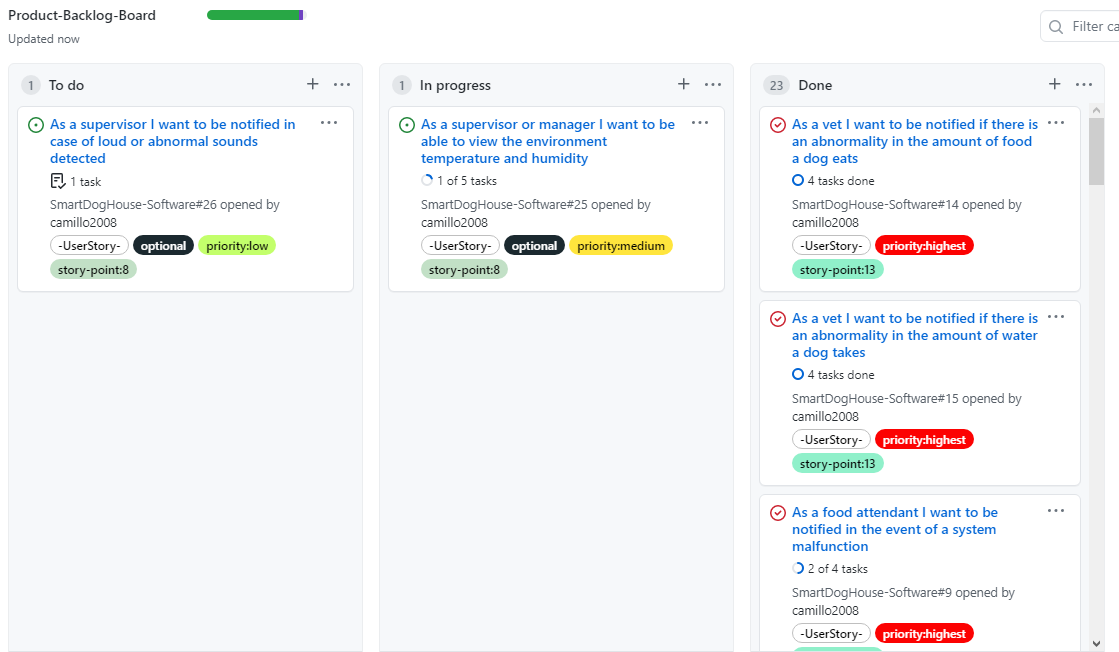
\includegraphics[width=1\textwidth]{Images/productBacklogBoard.png}
    \end{figure}
    All'inizio di ogni sprint, gli Item più importanti verranno inoltre eletti come Sprint Goals (COSA fare all'interno dello sprint). 
    Nel progetto gli item corrispondono uno a uno le User Stories, trasformate in Issue, con relativo tag, da risolvere durante gli sprint.Gli Item principali vengono raffinati iterativamente, quelli in cima infatti diverranno via via più specifici.
    
    All'interno delle repository invece sono stati incrementalmente implementate tante board quanti gli Sprint-Backlog. Vi sarà infatti una board per ogni Sprint. Non sono state usate le milestone per gli spint poichè nella piattaforma una issue può essere assegnata ad una sola milestone, mentre è possibile condividerla tra più board qualora non venisse completata in un solo Sprint.
    Le Sprint Backlog Boards tengono traccia degli specifici task da sviluppare all'interno dei singoli Sprint (COME raggiungere lo Sprint Goal) a partire dall/dagli Item selezionati. Le user stories selezionate dalla board del Product Backlog faranno parte anche della board per lo Sprint Backlog, assieme ai relativi raffinamenti. Gli Item principali vengono infatti raffinati iterativamente, quelli in cima diverranno via via più specifici.
    \begin{figure}[H]
        \caption{Sprint Backlog Board}
        \centering
       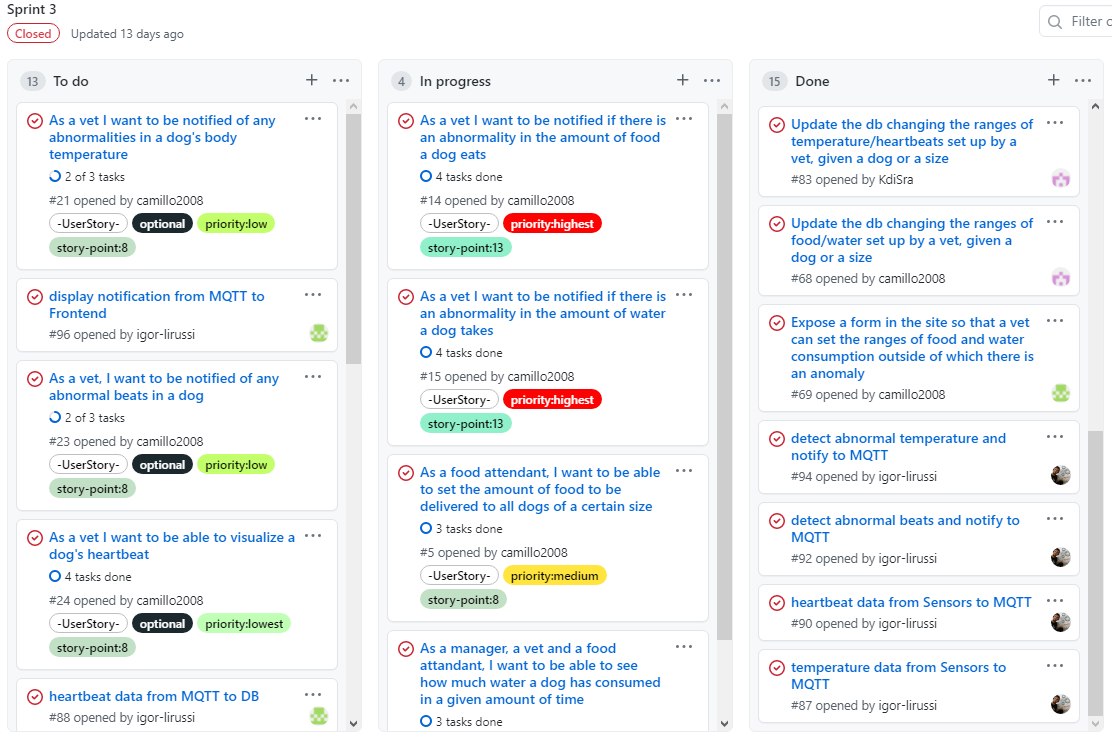
\includegraphics[width=1\textwidth]{Images/sprintBacklogBoard.png}
    \end{figure}
    I raffinamenti sono stati istanziati come altre issue, le quali vengono referenziate dalla user story principale, che acquisterà automaticamente in indicatore dei sottotask completati. Questo ci ha permesso di tenere traccia dell'andamento di uno sprint con granularità anche molto fine. Inoltre le sotto-issue possono essere condivise tra user-stories, evitando la ripetizione. Qualora una venga completata tramite l'aggiunta di una porzione di codice è possibile, tramite commit con sintassi closes \#NUMERO-ISSUE, chiudere in automatico la sotto-issue. Questa verrà inoltre spostata nella colonna \textit{Done}, e automaticamente l'indicatore dei task completati di una user-story avanzerà.
    Una volta completato la/le user-stories dello Sprint anche nel Product Backlog la relativa issue si sposterà nella colonna \textit{Done}. 
    Per il completamento dello Sprint Goal è stata considerata valida la "Definition of Done" specificata in precedenza.
    \begin{figure}[H]
        \caption{Milestone che descrivono i progressi della relazione}
        \centering
       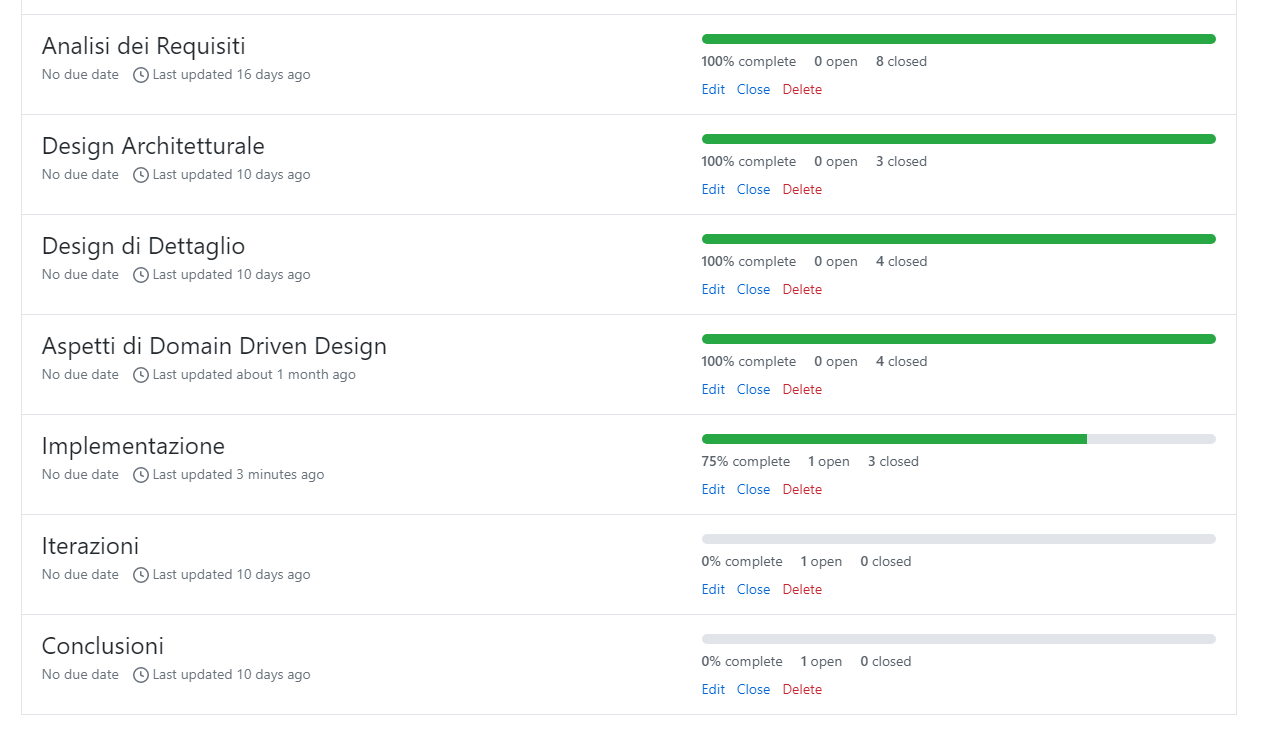
\includegraphics[width=1\textwidth]{Images/milestone_relazione.png}
    \end{figure}
    Una board aggiuntiva è stata creata per tenere traccia dei progressi della relazione. In questo caso ogni capitolo è stato definito come milestone, completabile alla scrittura di tutti i sottocapitoli, identificati come task, quindi issue, appartenenti alla relativa milestone.
    I vari task sono stati divisi in categorie standard per lo Scrum: \textit{"to Do", "in Progress", "Done"}.
    Qualora un sottocapitolo della relazione venga completato, tramite Overleaf è semplicemente possibile chiudere la relativa issue tramite il messaggio di commit visto in precedenza.
    Nel momento in cui un sottocapitolo viene chiuso, la relativa issue si sposta nella colonna \textit{Done} e il progresso relativo alla milestone del capitolo e dell'intero Report verrà aggiornato.
    In entrambi i tipi di board, relative agli sprint o alla relazione, è possibile aprire delle issue inerenti bug trovati, problemi alla sicurezza, o accorgimenti. Queste Issue compaiono nella board e possono venire assegnate a un componente specifico del gruppo affinchè se ne occupi.
    
    \paragraph{Telegram}
    Come strumento di messaggistica informale all'interno del gruppo, si è scelta la piattaforma Telegram. Accessibile facilmente da smartphone e da computer permette di aggiornare i componenti del gruppo immediatamente qualora vi siano delle urgenze. Il punto di forza rimane la  possibilità di spedire file di tutti i formati e di poter inserire nel gruppo dei BOT per automatizzare alcune azioni, tra cui le notifiche. Un'overview più chiara dell'utilizzo dei BOT per l'automatizzione verrà fornita nella \autoref{chap:CI}.
    \subparagraph{Bot per Sondaggi} Per facilitare la coordinazione quotidiana è stato creato un bot per inviare i sondaggi sul gruppo Telegram. Questo sia poiché il progetto è stato svolto prevalentemente a distanza, sia perché alcune parti necessariamente hanno richiesto la presenza di tutto il team.
    %immagine poll telegram
    \begin{figure}[H]
        \caption{Sondaggio giornaliero su Telegram}
        \centering
       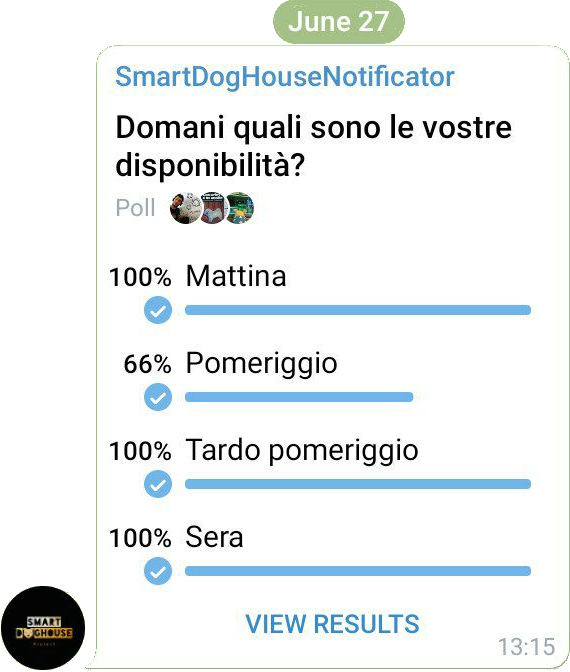
\includegraphics[width=0.4\textwidth]{Images/pollTelegram.png}
    \end{figure}
    
    \paragraph{Discord}
    Discord, nota piattaforma di comunicazione VoIP, è stato utilizzato invece come strumento di comunicazione formale. Si è creato un server apposito per il progetto, chiamato "SmartDogHouseChannel", con multiple stanze lavoro per diverse occasioni.
    I canali vocali sono stati utilizzati anche per la condivisione dello schermo, fattore chiave per la sincronizzazione e la comprensione senza dispendio non necessario di tempo. 

\section{Continuous Integration e Automatizzazione}
\label{chap:CI}
In questo capitolo si analizza la parte di integrazione e automatizzazione sia del progetto software che della relazione. 
    \subsection{Relazione di Progetto}
        Considerato che anche la relazione deve essere versionata e automatizzata, essendo parte del software e descrivendolo, abbiamo iniziato partendo da essa. 
        Come linguaggio di markup è stato scelto {\LaTeX}, per la sua flessibilità e potenza. 
        Come strumento per la compilazione invece è stato scelto Overleaf.com, poiché ha 3 vantaggi principali che il team ha individuato. Permette di collaborare sullo stesso progetto, in real-time, osservando i cambiamenti fatti dai collaboratori con la compilazione immediata, discutendone vocalmente i dettagli tramite la piattaforma di comunicazione VoIP. Permette inoltre di non dipendere da diversi IDE per {\LaTeX} installati in locale, che creerebbero conflitti e mismatch visuali. Infine permette di integrarsi con GitHub (solo Overleaf Professional), pushando i commit con i nomi desiderati in tutta fluidità direttamente dalla piattaforma web.
        Per incorporare gli elementi grafici più importanti si è fatto uso della piattaforma Draw.io. L'integrazione con GitHub è anche qui presente, permettendo di aprire il progetto e pushare le modifiche direttamente dal web. Inoltre è notevole il fatto che gli artefatti PNG abbiano essi stessi i metadati del progetto garantendo tre vantaggi. Il primo riguarda la non necessità di salvare un ulteriore file progetto rispetto all'artefatto. Il secondo riguarda la possibilità di aprire direttamente i PNG e poter fare le modifiche desiderate. Il terzo è l'intrinseco versionamento pure dei progetti assieme ai PNG. 
        Per le grafiche dove è necessaria più una collaborazione real-time dei membri del team, con schemi inerenti al DDD più esotici, oppure ove è più presente il contatto con il cliente, la scelta è ricaduta sulla piattaforma Miro.
        Nel repository, tramite l'utilizzo di GitHub Actions, è stato implementato un processo di automatizzazione con multipli Job. 
        
        Il primo Job si attiva ad ogni push ricevuta, compila il Latex per mezzo di una action e, qualora si verificassero degli errori, li salva in un log più piccolo, che verrà caricato come artefatto. Invece, se nessun errore è presente, è il pdf generato a venire caricato come artefatto.
        
        La terminazione di questo Job attiva altri due Job, dipendenti, che si occupano delle notifiche Telegram. Anche qui per mezzo di una action viene mandato un messaggio di notifica sul gruppo, sia se la build del Latex abbia avuto successo, sia che ci siano stati errori. In caso di fallimento assieme al messaggio viene inoltrato sul gruppo pure il log conciso che contiene solo gli errori Latex. 
        
        Per la gestione delle release è stato inoltre implementato un altro Job che verifica se nel messaggio di commit è presente uno speciale segnalatore -TAG{}. Nel caso sia presente vuol dire che è stato specificato un tag manualmente, ciò può avvenire qualora si voglia far avanzare la versione Major o Minor avendo fatto cambiamenti significativi.
        La scelta di permettere la numerazione dei tag a mano è stata dettata dalla necessità di controllo e cusotomizzazione di questi ultimi: in una relazione si vuole scegliere quando effettuare la release e, adottando il semantic versioning, il grado di cambiamento che si ritiene più opportuno.
        Qualora non venisse specificato un tag, in automatico viene incrementato l'ultimo numero (bugfix) del semantic versioning.
        
        Il Job successivo si occupa del deploy, e viene attivato solamente se è stato generato correttamente il tag nella parte precedente. Questo Job scarica il pdf precedentemente generato negli artefatti e si occupa di farne una release con nome coerente e con il tag specificato. 
        
        Al termine della release vengono lanciati altri due Job, anch'essi dipendenti, che si occupano di notificarne il completamento. 
        Il primo usa una GitHub Actions per inoltrare una mail ai componenti del gruppo contenente il pdf della release. Per fare ciò si è dovuto creare un account Gmail specifico che funge da casella di invio. Si può inoltre sfruttare come account di notifica per un'eventuale newsletter agli iscritti ad ogni nuova release. 
        Il secondo Job si occupa parallelamente di inoltrare un messaggio Telegram sul gruppo dei developers contenente anch'esso il pdf della release, il responsabile e il testo del commit. 
        %immagine push telegram
        \begin{figure}[H]
            \caption{Avviso di push su Telegram}
            \centering
           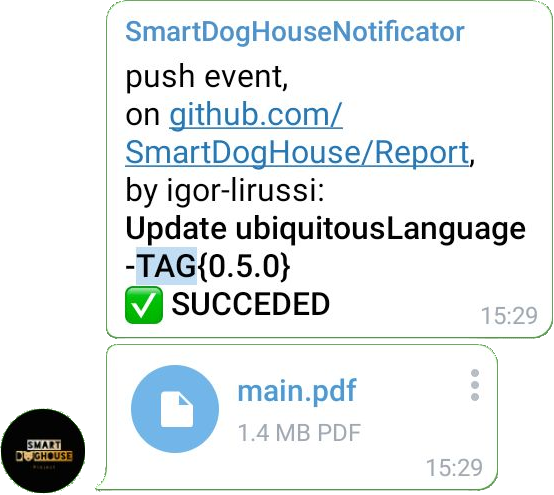
\includegraphics[width=0.4\textwidth]{Images/pushTelegram.png}
        \end{figure}
        Un ultimo Job è stato creato per gestire anche le GitHub Pages, le quali forniscono un sito in cui consultare la relazione online. Per fare ciò è stato creato un nuovo branch sul quale viene fatto il commit dei file Html generati grazie a Pandoc.
        In conclusione sarà possibile consultare questo report sia in versione pdf automaticamente generata ad ogni cambiamento, che direttamente via sito web, prodotto dai sorgenti.
        %TABELLA PIPELINE CI REPORT
        \begin{figure}[H]
            \caption{Pipeline implementata per l'esecuzione di un commit con release-tag}
            \centering
            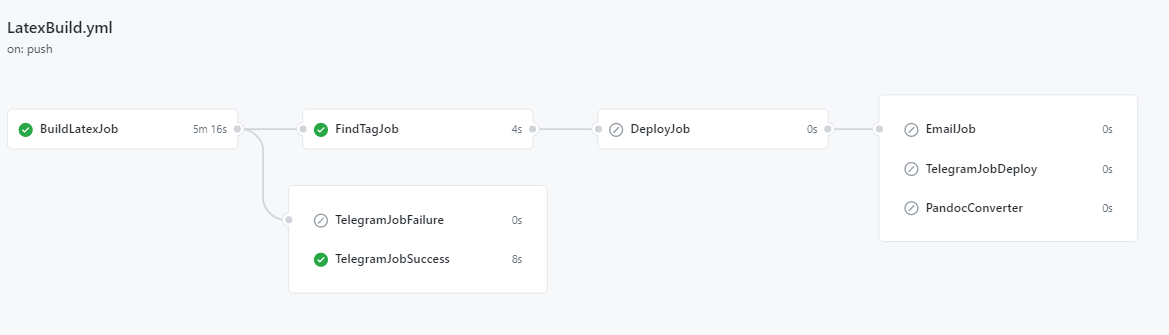
\includegraphics[width=1\textwidth]{Images/RepoCI.png}
        \end{figure}
        
        \subparagraph{Tool utilizzati}
        \begin{itemize}
            \item HackMD
            \item Overleaf
            \item Draw.io
            \item Miro (\href{https://miro.com/app/board/o9J_lEyTG7Q=/}{link alla board})
            \item GitHub Actions
            \item Telegram Bots
            \item Pandoc
            \item GitHub Pages
        \end{itemize}

    \subsection{Progetto}
        Riguardo al software del progetto, sono stati utilizzati parecchi linguaggi di programmazione differenti, quindi le soluzioni adottate variano in base alle implementazioni e all'importanza relativa. Di seguito si riporta una linea generale implementata nel repository principale per il software, poi seguita anche dagli altri repository, con dovute eccezioni in base alle limitazioni dei linguaggi.
        Avendo usato Python (e il suo derivato MicroPython) per le parti principali non è stato necessario un vero e proprio strumento di build, in quanto basta un'interprete per far girare il codice.
        Particolare attenzione è stata fatta ai test, implementati tramite \textit{unittest} in un package dedicato. Tramite il compando \textit{discover} tutti i test implementati vengono eseguiti in maniera automatica. Ciò ha permesso di scoprire parecchi bug prima di rilasciare il codice online. La procedura è stata automatizzata sfruttando la CI di GitHub Actions, la quale fallisce se i test non vengono eseguiti correttamente. 
        
        \subsubsection{Utilizzo Stub per il Testing Automatico}
        Si è fatto ricorso agli stub data la necessità di testare il codice per i microcontrollori e l'impossibilità di poterlo testare in maniera totalmente automatica su di essi. Infatti, la soluzione ideale per comodità e qualità è di poter eseguire i test su un normale computer, automatizzando il tutto in cloud. Tuttavia, per poter testare il codice Micropython devono essere presenti le classi che il firmware mette a disposizione quando installato sui microcontrollori. Purtroppo non è possibile installare il firmware su un computer, il che rende normalmente impossibile eseguire e testare il codice. 
        Per ovviare al problema sono stati inseriti nel codice della repository degli stub che permettono di simulare il firmware installato sulla macchina fisica e il comportamento dei rispettivi sensori e attuatori. Gli Stub purtroppo devono essere inseriti a livello del codice, in quanto un'altra posizione modificherebbe i percorsi di import e il codice non sarebbe più eseguibile sul microcontrollore. In questo modo è possibile verificare continuamente il codice scritto attraverso i test eseguiti automaticamente sul repository. Un messaggio Telegram viene mandato anche qui sul gruppo dei developer per segnalarne l'esito.
        
        \subsubsection{Coverage} Eseguiti i test è buona norma osservare la coverage di questi. In questo caso per Python è stato usato il pacchetto \textit{coverage}, questo permette di generare la coverage dei test e il relativo sito web. Tramite GitHub Actions e GitHub Pages questo è stato messo online, per una rapida consultazione. Eventualmente è anche stata generata la coverage in xml per siti come CodeCov, i quali permettono di ottenere anch'essi un resoconto ordinato. La coverage creata viene pubblicata per entrambi i branch main e develop.
        
        \subsubsection{Documentazione} Il codice è stato documentato per assicurare la qualità. Il pacchetto \textit{pdoc} usato per il repo principale permette di generare la documentazione html a partire dai sorgenti. Anche qui è stato automatizzata la creazione e il deploy del sito web tramite GitHub Actions e GitHub Pages per facilitarne la consultazione. 
        
        \subparagraph{Versioning and Deployment} Anche in questo caso, come nel report, il versioning è automatico, con la possibilità di controllo manuale. Qualora non venga specificato un tag nel commit la CI implementata di GitHub Actions genera un tag con la versione bugfix incrementata di uno. Qualora un tag venisse specificato il progetto si porta avanti a quella versione. Ciò ha reso molto preciso e veloce il versionamento del nostro software in caso di cambiamenti minimi o estesi.
        Il deploy del software viene fatto puntualmente in automatico con la versione elaborata all'interno delle Releases di GitHub.
        
        \subparagraph{Quality Assurance}
        Per quanto riguarda la parte di quality assurance, la scelta è ricaduta su tre servizi di aziende completamente diverse: Sonarcloud, Codacy e Codefactor. I relativi servizi offrono un'analisi della qualità codice completamente gratuita per il piano base. La scelta di diversificare i fornitori del servizio è motivata da due ragioni. La prima è che sono state riscontrate interruzioni e bug nei corrispettivi siti, la diversificazione offre una copertura 24/7. La seconda ragione consiste nel fatto che ognuno offre solo alcune misurazioni sul codice tra Maintainaility, Issues, Complexity, Duplicaizione, Coverage, Security, Vulnerabilities, Bugs. Usare tre sevizi offre in conclusione una copertura maggiore sulla qualità. Qualora le pull request o il codice del repo non soddisfi gli standard ciò permette di immediata individuazione. 
        Per l'aggiornamento delle dipendenze è stato attivato Dependabot su tutti i repository, questo permette di ottenere delle pull-request in automatico qualora venisse individuato un possibile aggiornamento.
        
        \subparagraph{Tool utilizzati}
        \begin{itemize}
            \item Test/Coverage/Documentation Software
            \item GitHub Actions
            \item GitHub Pages
            \item Telegram Bots
            \item Dependabot
            \item Sonarcloud/Codacy/Codefactor
        \end{itemize}








